\documentclass[12pt]{article}
\usepackage[margin=1in]{geometry}
\usepackage{graphicx}
\usepackage{booktabs}
\usepackage{amsmath}
\title{The Effect of Paid Search Advertising on Revenue: \\
	A Replication of the eBay Natural Experiment}
\author{Hunter Massey}
\date{\today}
\begin{document}
\maketitle

\section{Introduction}
This paper studies the causal effect of paid search advertising on eBay’s revenue. Firms spend billions of dollars each year on search engine marketing (SEM), yet measuring the true return on these expenditures is difficult because advertising exposure is typically correlated with consumer demand. In other words, firms tend to advertise more in markets or periods where demand is already high, making simple correlations misleading. Blake, Nosko, and Tadelis (2014) provide a rare opportunity to estimate a causal effect through a natural experiment in which eBay temporarily turned off paid search advertising in selected markets. In this replication, I use a difference-in-differences (DID) framework to estimate how revenue changed when paid search ads were shut off in treatment markets relative to control markets.


\section{Experimental Setting}
In May 2012, eBay stopped bidding on Google AdWords in 65 of its 210 designated market areas (DMAs). The advertising shutdown began on May 22 and lasted approximately eight weeks. These 65 DMAs form the treatment group (where \texttt{search\_stays\_on = 0}), while the remaining DMAs continued advertising and serve as the control group (\texttt{search\_stays\_on = 1}). The goal of the experiment was to measure how much revenue would decline if paid search advertising were eliminated.

Importantly, the treatment was not fully randomized. The largest DMAs were excluded from the treatment group, meaning that treatment and control markets differed in baseline revenue levels. Because of these pre-existing differences, a simple comparison of average revenue between treatment and control groups would be biased. Instead, the appropriate approach is a difference-in-differences strategy that compares the change in revenue before and after May 22 across the two groups. This approach accounts for time-invariant differences between markets and isolates the treatment effect from common time trends.


\section{Data and Figures}
The dataset contains daily revenue observations for 210 DMAs from April through July 2012. Each observation includes the date, DMA identifier, an indicator for treatment period (pre- or post-May 22), group assignment (treatment or control), and revenue. I construct log revenue to stabilize variance and interpret differences as approximate percentage changes.


\begin{figure}[h]
	\centering
	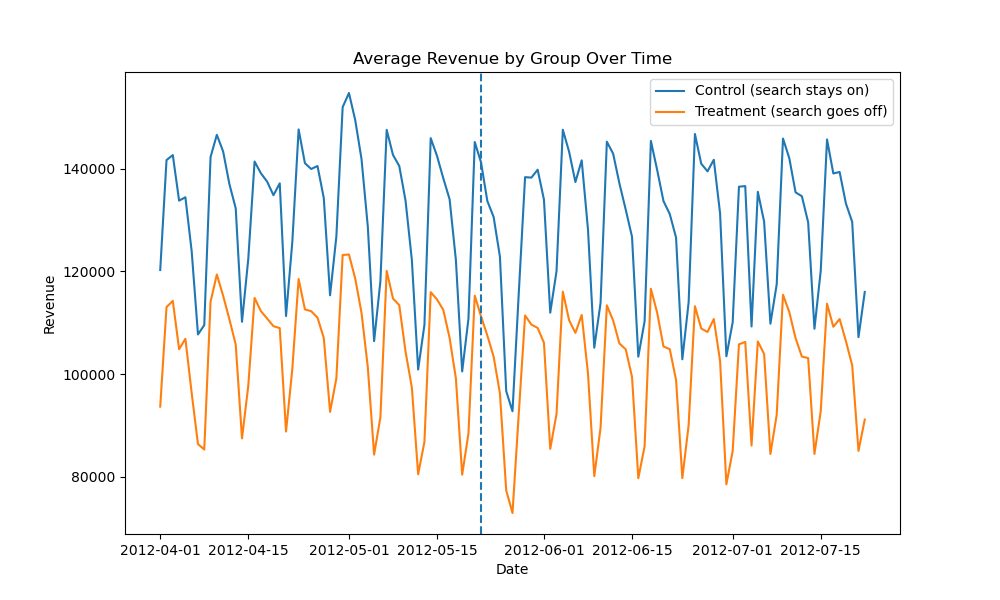
\includegraphics[width=0.85\textwidth]{../output/figures/figure_5_2.png}
	\caption{Average revenue for treatment and control DMAs over time.
		The dashed line marks May 22, 2012, when SEM was turned off
		for the treatment group.}
	\label{fig:revenue}
\end{figure}

Figure \ref{fig:revenue} plots average daily revenue for treatment and control DMAs over time. The control group consistently has higher average revenue, which is expected since the largest DMAs were excluded from treatment. Both groups display similar weekly oscillation patterns, reflecting common seasonal demand fluctuations. Visually, it is difficult to detect a clear break in revenue at the treatment date, suggesting that any effect of turning off paid search may be small.

\begin{figure}[h]
	\centering
	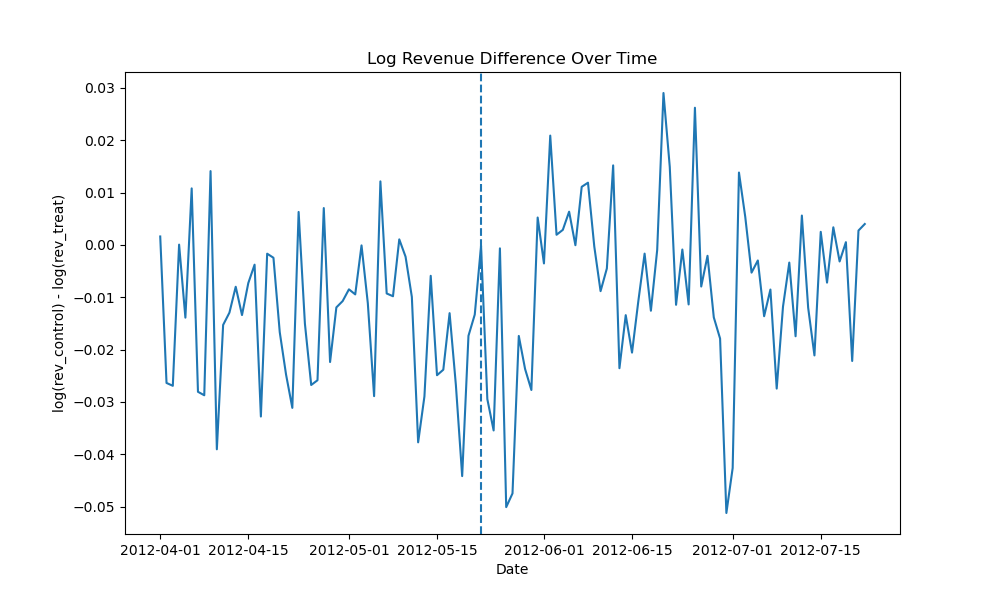
\includegraphics[width=0.85\textwidth]{../output/figures/figure_5_3.png}
	\caption{Log-scale average revenue difference between control and treatment
		groups over time. The gap appears to increase after May 22.}
	\label{fig:logdiff}
\end{figure}

Figure \ref{fig:logdiff} shows the difference in log average revenue between control and treatment groups over time. Before May 22, the log revenue gap fluctuates around a relatively stable level. After the treatment begins, the gap appears to widen slightly, indicating that treatment DMAs may have experienced a small relative decline in revenue. However, the change is subtle and not visually dramatic, motivating a formal DID estimation to quantify the effect.

\section{Results}

\input{../output/tables/did_table.tex}

The difference-in-differences estimate is $\hat{\gamma} = -0.0066$ in log scale. Interpreted in levels, this corresponds to $\exp(-0.0066) = 0.9934$, meaning that turning off paid search reduced revenue by approximately 0.66 percent in the treated DMAs. While the point estimate is negative, the 95\% confidence interval $[-0.0175, 0.0043]$ includes zero. This implies that the effect is not statistically significant at the 5 percent level.

Economically, the results suggest that paid search advertising had only a very small impact on revenue during this experiment. For a well-known brand like eBay, many consumers likely navigate directly to the site or find it through organic search results. As a result, paid search ads may largely capture inframarginal customers who would have purchased anyway. These findings are consistent with the main conclusions of Blake et al. (2014).


\section{Conclusion}

This replication uses a difference-in-differences framework to estimate the effect of turning off paid search advertising on eBay’s revenue. The estimated effect is small and statistically insignificant, implying that paid search advertising had limited incremental impact during the experimental period. This result aligns with the original findings of Blake et al. (2014).

There are several limitations to this analysis. The data provided are scaled rather than actual revenue figures, the treatment was not fully randomized, and the estimation approach is a simple DID rather than a regression with additional controls. Nevertheless, the results highlight an important lesson for marketing analytics: large advertising expenditures do not necessarily translate into meaningful incremental revenue, particularly for established brands.

\begin{thebibliography}{9}
\bibitem{blake2014}
Blake, T., C. Nosko, and S. Tadelis (2014).
``Consumer Heterogeneity and Paid Search Effectiveness: A Large-Scale Field Experiment.''
\textit{Econometrica}, 83(1): 155--174.
\bibitem{taddy2019}
Taddy, M. (2019).
\textit{Business Data Science}. McGraw-Hill, Chapter 5.
\end{thebibliography}
\end{document}

